\chapter{Analysis}

Measurement results / analysis / discussion: 1/3

\begin{itemize}
\item whatever you have done, you must comment it, compare it to other systems, evaluate it
\item usually, adequate graphs help to show the benefits of your approach
\item caution: each result/graph must be discussed! what's the reason for this peak or why have you ovserved this effect
\end{itemize}

\section{Transmitted image size}
\begin{figure}[H]
\centering
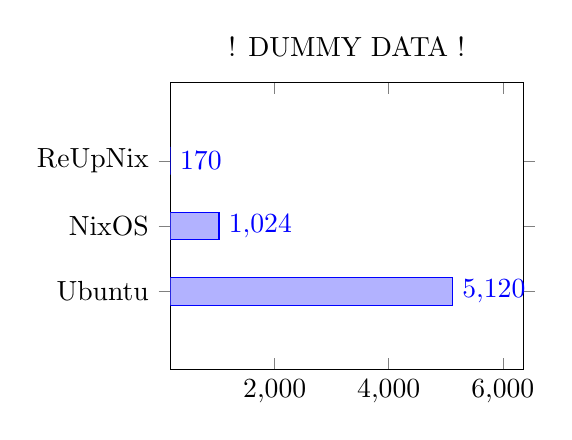
\begin{tikzpicture}
  \begin{axis}[
    title  = ! DUMMY DATA !,
    xbar,
    ytick             = data,
    enlarge y limits  = 0.6,
    enlarge x limits  = { 0.25, upper},
    width = 0.5\textwidth,
    symbolic y coords = {Ubuntu, NixOS, ReUpNix},
    nodes near coords,
  ]
  \addplot coordinates { (170,ReUpNix)         (1024,NixOS)
                         (5120,Ubuntu)   };
  \end{axis}
\end{tikzpicture}
\caption{Image size by OS in megabytes}
\end{figure}
\clearpage
\section{Image Size}
We compared \textit{reUpNix}, \textit{NixOS}, Ubuntu 22.04, and
\textit{Yocto Kirkstone} by their image size, with the methodology introduced
in chapter XXX. All system images feature an \ac{OCI}-compliant container runtime,
and the Azure IoT Edge runtime (Variation 1). Additionally, each system has a
variation with the \ac{ADU} Agent installed (Variation 2). The results are shown
in figure XXX.
\begin{table}[H]
	\centering
	\begin{tabular}{l|l|l|l|l}
	\toprule
		Operating System & Image Variation 1 & $\Delta$ & Image Variation 2 & $\Delta$\\
	\midrule
    \textbf{reUpNix} & \text{1 289 MB} & \color{ba-green}{- 1 010 MB} &  \text{- MB} & a\\
    \textbf{NixOS 23.01} & \text{2 361 MB} & \textcolor{ba-red}{+ 62 MB} & \text{- MB} & a\\
    \textbf{Ubuntu 22.04} & \text{2 299 MB} & \text{-} & \text{2 311 MB} & \text{-}\\
    \textbf{Yocto Kirkstone} & \text{- MB} & a &\text{- MB} & a\\
	\bottomrule
	\end{tabular}
	\caption{Image size by OS for each variation}
	\label{tab:si-in-tables}
\end{table}
\begin{figure}[H]
\centering
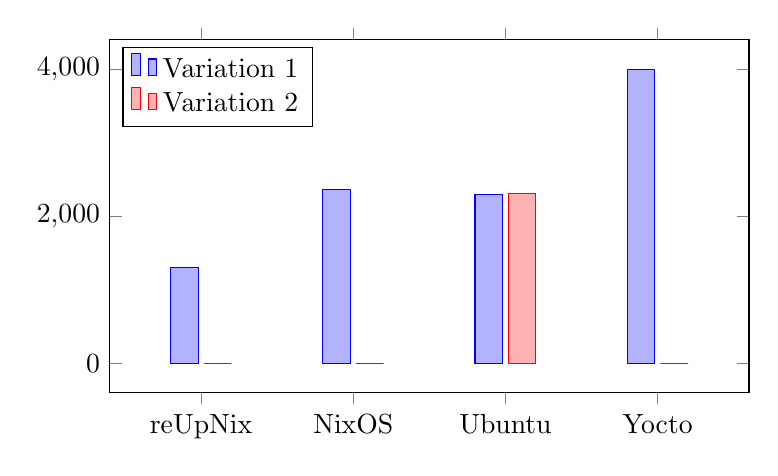
\begin{tikzpicture}

  \begin{axis}[
    ybar,
    xtick             = data,
    width = 0.8\textwidth,
    height = 0.5\textwidth,
    enlarge x limits  = 0.2,
    symbolic x coords = {reUpNix, NixOS, Ubuntu, Yocto},
    legend style={at={( 0.02,0.98)},anchor=north west}
  ]
  \addplot coordinates { (reUpNix,1305.782) (NixOS,2364.346) (Ubuntu, 2299.894) (Yocto, 4000)};
  \addplot coordinates { (reUpNix,0) (NixOS, 0) (Ubuntu, 2311.166) (Yocto, 0)};
  \legend{Variation 1, Variation 2}
\end{axis}
\end{tikzpicture}
\caption{Image size by OS in Megabytes}
\end{figure}
We can see that with its 1305 Megabytes \textit{reUpNix} has a 43\% smaller image size
than Microsoft's recommended Ubuntu 22.04. Further, the difference in image size
between Ubuntu 22.04 and \textit{NixOS} is only 64 Megabytes.
Finally, the difference between the Variation 1 and Variation 2 is almost
negligible across all operating systems, since the \ac{ADU} Agent is small in
size, and features no additional dependencies.

\section{Mean time to recover}
\begin{figure}[H]
\centering
\begin{tikzpicture}
  \begin{axis}[
    title  = ReUpNix,
    ybar,
    enlarge y limits  = {0.15,upper},
    width = 0.5\textwidth,
    nodes near coords,
  ]
    \addplot table [x=seconds, y=times, col sep=comma] {data/time-to-recover-reupnix.csv};
  \end{axis}
\end{tikzpicture}
\begin{tikzpicture}
  \begin{axis}[
    title  = NixOS,
    ybar,
    enlarge y limits  = {0.15,upper},
    width = 0.5\textwidth,
    nodes near coords,
  ]
    \addplot table [x=seconds, y=times, col sep=comma] {data/time-to-recover-nixos.csv};
  \end{axis}
\end{tikzpicture}
\begin{tikzpicture}
  \begin{axis}[
    title  = Ubuntu 22.04,
    ybar,
    enlarge y limits  = {0.15,upper},
    width = 0.5\textwidth,
    nodes near coords,
  ]
    \addplot table [x=seconds, y=times, col sep=comma] {data/time-to-recover-ubuntu.csv};
  \end{axis}
\end{tikzpicture}
\caption{Time of recovery after a reboot by OS in seconds.}
\end{figure}
